\section{Classes}

\subsection{Position}
La classe position permet de positionner ou d'obtenir la position d'un
�l�ment, elle contient aussi diff�rentes donn�es par rapport � l'orientation.
\begin{figure}[htbp]
\begin{center}
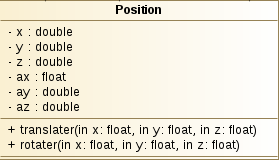
\includegraphics[width=7cm]{../images/class/position.png}
\end{center}
\label{fig:figure}
\caption{Classe Position}
\end{figure}


\newpage
\subsection{Diagramme complet}
\begin{figure}[htbp]
\begin{center}
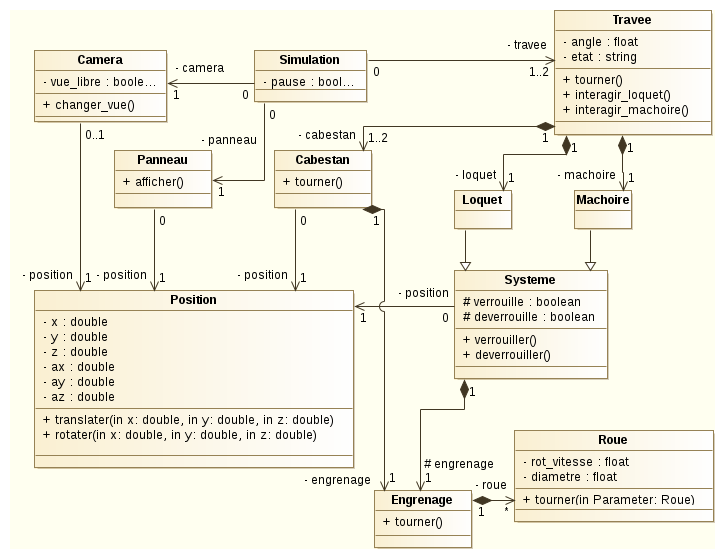
\includegraphics[width=15cm]{../images/class/class.png}
\end{center}
\label{fig:figure}
\caption{Diagramme de classe global}
\end{figure}
